% Template: LaTeX file for ICMC 2009 papers, with hyper-references
%
% derived from the DAFx-06 templates
%
% 1) Please compile using latex or pdflatex.
% 2) Please use figures in vectorial format (.pdf); .png or .jpg are working otherwise 
% 3) Please use the "papertitle" and "pdfauthor" commands defined below

%------------------------------------------------------------------------------------------
\documentclass[twoside,10pt]{article}
\usepackage{icmc2009,amssymb,amsmath} 
%\setcounter{page}{1}

\usepackage{mathptmx} 

%____________________________________________________________
%  !  !  !  !  !  !  !  !  !  !  !  ! user defined variables  !  !  !  !  !  !  !  !  !  !  !  !  !  !
%==== set the title ====
\def\papertitle{DBAP - Distance-Based Amplitude Panning}
%\def\papertitle{}	%-- should be empty for the submission anyway!

%==== 1st submission: author name and affiliation are empty for anonymous submission ====
%\def\paperauthorA{} 
%\affiliation{}{}


%==== final submission: author name and affiliation ====
%---- uncomment 1 to 4 lines, for 1 to 4 authors
\def\paperauthorA{Trond Lossius}
\def\paperauthorB{Pascal Baltazar}
\def\paperauthorC{Th\'eo de la Hogue}
%\def\paperauthorD{Fourth Author}

%%---- set correspnding affiliation data for...
%%-- 1 author
\twoaffiliations{\paperauthorA}{BEK\\C. Sundtsgt. 55\\5004 Bergen\\Norway\\trond.lossius@bek.no}
%%-- 2 authors with same affiliation
{\paperauthorB, \paperauthorC}
{GMEA\\4 rue Sainte Claire\\81000 Albi\\France \\pb@gmea.net, theod@gmea.net}

%-- 2 authors with different affiliations
%\twoaffiliations{\paperauthorA}{School\\ Department}
%  {\paperauthorB}{Company\\ Address}

%%-- 3 authors with different affiliations
%\threeaffiliations{\paperauthorA}{BEK\\C. Sundtsgt. 55\\5004 Bergen\\Norway\\trond.lossius@bek.no}
%  {\paperauthorB}{GMEA\\4 rue Sainte Claire\\81000 Albi\\France\\pb@gmea.net}
%  {\paperauthorC}{GMEA\\4 rue Sainte Claire\\81000 Albi\\France\\theod@gmea.net}

%%-- 4 authors with different affiliations
%\fouraffiliations{\paperauthorA}{School A\\ Department X}
%  {\paperauthorB}{Company\\ Address}
%  {\paperauthorC}{School B\\ Department Y}
%  {\paperauthorD}{School C\\ Department Z}

%  ^  ^  ^  ^  ^  ^  ^  ^  ^  ^ user defined variables  ^  ^  ^  ^  ^  ^  ^  ^  ^  ^  ^  ^ 
%------------------------------------------------------------------------------------------

%%-- if using .ps or .eps figure files, they will be converted on the fly
%%-- RMK: for faster LaTeX runs, use it only once after adding new \includegraphics[]{} cmds
%\usepackage{epstopdf}	 

%---- the hyperref package must be last to properly work
\usepackage[pdftex,
       pdftitle={\papertitle},
	pdfauthor={\paperauthorA},
	colorlinks=false,bookmarksnumbered,pdfstartview=XYZ]{hyperref}
%\pdfcompresslevel=9
\usepackage[pdftex]{graphicx}	% for compatible graphics with hyperref
\usepackage[figure,table]{hypcap}	% corrects the hyper-anchor of figures/tables

\title{\papertitle}

\hyphenation{pan-ning-based}
\sloppy

%------------------------------------------------------------------------------------------
\begin{document}

\DeclareGraphicsExtensions{.png,.jpg,.pdf} % used graphic file format for pdflatex
    
\maketitle




%%%%%%%%%%%%%%%%%%%%%%%%%%%%%%%%%%%%%%%%%%%%%%%%%%%%%%%%%
%
% Abstract
%
%%%%%%%%%%%%%%%%%%%%%%%%%%%%%%%%%%%%%%%%%%%%%%%%%%%%%%%%%


\begin{abstract}
Most common techniques for spatialization require the listener to be positioned at a ``sweet spot'' surrounded by loudspeakers. For practical concert, stage, and installation applications such layouts may not be desirable. Distance-based amplitude panning (DBAP) offers an alternative panning-based spatialization method where no assumptions are made concerning the layout of the speaker array nor the position of the listener.  DBAP is implemented both as an external for Max/MSP and as a module for the Jamoma Modular framework.
\end{abstract}








%%%%%%%%%%%%%%%%%%%%%%%%%%%%%%%%%%%%%%%%%%%%%%%%%%%%%%%%%
%
% Introduction
%
%%%%%%%%%%%%%%%%%%%%%%%%%%%%%%%%%%%%%%%%%%%%%%%%%%%%%%%%%


\section{Introduction}\label{sec:introduction}

Multichannel and surround sound reproduction is becoming common for both consumer applications as well as musical and artistic purposes. A number of spatialization techniques exist for virtual positioning of sound sources using an array of loudspeakers. These often assume that the position of the listener is known and fixed, and that the speakers are surrounding the listener either on a two-dimensional ring or a three-dimensional sphere. Examples of such speaker layouts and spatialization techniques are stereo panning, ITU 5.1 surround \cite{ITU:1993_surround_5:1}, further extended industrial multichannel configurations \cite{Rumsey:2001spatial_audio}, vector-based amplitude panning (VBAP) \cite{Pulkki:1997vbap}, and first- and higher-order ambisonics \cite{Gerzon:1974surround, Poletti:2000holographic_sound}.

Wave field synthesis (WFS) and Virtual Microphone Control (ViMiC) \cite{Peters:2008vimic} are noticeable exceptions to the aforementioned ``sweet spot'' restriction.

WFS reproduces signals in a large listening area. The spatial properties of the acoustical scene can be perceived correctly by an arbitrarily large number of listeners regardless of their position inside this area \cite{Spors:2004sound_field_synthesis}. Due to the high number of loudspeakers required, WFS might be impractical to use for financial reasons and time constraints unless one is working on a site where a permanent setup resides.

ViMiC incorporates distance-based signal delays between speakers, simulation of microphone patterns, early reflections, and surface absorption. This makes it relatively CPU-intensive.  Thus ViMiC may require a dedicated computer for spatialization or restrictions on the number of loudspeakers used as compared to other techniques.

For real-time music and sound purposes, the low CPU requirements of matrix-based spatialization techniques make them popular choices. VBAP as well as ambisonics are readily available for use in common software environments for real-time processing such as Max/MSP \cite{Pulkki:2000vbap_max, Schacher:2006ambi_max, Neukom:2008ambipan}, but they require that the listeners are restricted to a relatively small listening area surrounded by loudspeakers arranged in a circle or sphere.  These requirements may not be feasible or desired in practical applications.  

Distance-based amplitude panning (DBAP) is a matrix-based spatialization technique that takes the actual positions of the speakers in space as the point of departure, while making no assumptions as to where the listeners are situated. This makes DBAP useful for a number of real-world situations such as concerts, stage productions, installations\cite{lossius:2008installations}, and museum sound design where predefined geometric speaker layouts may not apply.


%%%%%%%%%%%%%%%%%%%%%%%%%%%%%%%%%%%%%%%%%%%%%%%%%%%%%%%%%
%
% Fundamentals
%
%%%%%%%%%%%%%%%%%%%%%%%%%%%%%%%%%%%%%%%%%%%%%%%%%%%%%%%%%

\section{Distance-based amplitude panning}

\subsection{Fundamentals}

\textit{Distance-based amplitude panning (DBAP)} extends the principle of equal intensity panning from a pair of speakers to a loudspeaker array of any size, with no \textit{a priori} assumptions about their positions in space or relative to each other.
For simplicity, the method will be discussed using a two-dimensional model. This can be readily extended to three dimensions.

The Cartesian coordinates of a virtual source is given as $(x_{s}, y_{s})$. For a model with $N$ speakers, the position of the $i$th speaker is given as $(x_{i}, y_{i})$. The distance $d_{i}$ from a source to each of the speakers is

\begin{equation} \label{eq:distance}
d_{i} = \sqrt{ {(x_{i} - x_{s})}^2 + {(y_{i} - y_{s})}^2 } \qquad \textrm{for } 1 \leq i \leq N \textrm{ .}
\end{equation}

For simplicity, the source is presumed as having unity amplitude. DBAP then makes two assumptions. The first is that intensity is to be constant regardless of the position of the virtual source. This can be considered an extension of the principle of constant intensity stereo panning to multiple channels. If the amplitude of the $i$th speaker is $v_{i}$, this implies

\begin{equation} \label{eq:constant_intensity}
I = \sum_{i=1}^{N} {v_{i}}^2 = 1 \textrm{ .}
\end{equation}

Secondly, it is assumed that all speakers are active at all times, and the relative amplitude of the $i$th speaker relates to the distance from the virtual source as 

\begin{equation} \label{eq:inverse_distance}
v_{i} = \frac{k}{2 d_{i} a} \textrm{ ,}
\end{equation}

where $k$ is a coefficient depending on the position of the source and all speakers, while $a$ is a coefficient calculated from the rolloff $R$ in decibels per doubling of distance:

\begin{equation} \label{eq:rolloff}
	a = 10^{\frac{-R}{20}}
\end{equation}

A rolloff of $R = 6$ dB equals the inverse distance law for sound propagating in a free field. For closed or semi-closed environments $R$ will generally be lower, in the range 3-5 dB, and depend on reflections and reverberation \cite{Everest:2000handbook_acoustics} (pp. 84-88). Equation (\ref{eq:rolloff}) then represents a simplified description of attenuation with distance, but simulation of reflections and reverberation is anyway beyond the scope of an amplitude-panning based spatialization method.

Combining equations (\ref{eq:constant_intensity}) and (\ref{eq:inverse_distance}) $k$ can be found as:

\begin{equation} \label{eq:calculate_k}
k = \frac{2a}{\sqrt{\sum_{i=1}^{N} \frac{1}{{d_{i}}^2}}}
\end{equation}




\subsection{Spatial Blur}

If the virtual source is located at the exact position of one of the loudspeakers, (\ref{eq:calculate_k}) will cause a division by zero. Combining equations (\ref{eq:inverse_distance}) and (\ref{eq:calculate_k}) we get

\begin{equation}
v_{j} = \frac{1}{\sum_{i=0}^{N} \frac{{d_{j}}^2}{{d_{i}}^2}}
\end{equation}

From this it can be shown that

\begin{equation} \label{eq:distance_zero}
\lim_{d_{j} \rightarrow 0} v_{i} = 
\left\{ \begin{array}{ll} 
1 & \textrm{if $i=j$}\\ 
0 & \textrm{if $i \ne j$}
\end{array} \right.
\end{equation}

When the virtual source is located at the exact position of one of the loudspeakers, only that speaker will be emitting sound. This may cause unwanted changes in spatial spread and coloration of a virtual source in a similar way as observed for VBAP \cite{Pulkki:1999vbap}. To adjust for this \textit{spatial blur} $r_{s} \ge 0$ is introduced in equation (\ref{eq:distance}):

\begin{equation} \label{eq:mod_distance}
d_{i} = \sqrt{ {(x_{i} - x_{s})}^2 + {(y_{i} - y_{s})}^2 + {r_{s}}^2}
\end{equation}

In two dimensions blur can be understood as a vertical displacement between source and speakers. The larger $r$ gets, the less the source will be able to gravitate towards one speaker only. Practical experience indicates that there is a limit to the amount of blur that can be applied, or the precedence effect \cite{Litovsky:1999precedence_effect} will come into play, causing the perceived direction of the source to gravitate towards the speaker(s) closest to the listener.

In the implementations of DBAP discussed in section \ref{sec:implementation} the blur coefficient is normalized, using the covariance of distance from centre of loudspeaker rig to loudspeakers as scaling factor, in order to make the blur coefficient less sensitive to changes in size of loudspeaker layouts.



\subsection{Sources Positioned Outside the Field of Speakers}

The model presented so far is not able to cater for sources located outside the field of speakers. As distance to the field increases, the relative difference in distance from source to each of the speakers diminishes, resulting in progressively less difference in levels between the speakers, much the same way as when increasing spatial blur. Compensating for this requires additional calculations.

First, the \emph{convex hull} of the field of loudspeakers is calculated. In two dimensions the convex hull ``is the shape taken by a rubber band stretched around nails bounded into the plane at each point'' \cite{Rourke:1998_geometry}. It is then determined if the source is outside the hull or not. If it is inside or on the boundary no additional steps need to be taken. If the source is located outside, then the projection of the source onto the boundary of the hull is calculated, defined as the point on the boundary with the shortest possible distance to the source. This source position is  substituted for its projection in subsequent calculations. In addition, the distance from source to the convex hull is returned. This value can be used for optional added spatial processing such as gain attenuation, air filtering, Doppler effect, or gradual introduction of reverb with increasing distance from the hull.


\subsection{Extending DBAP by Introducing Speaker Weights}

% CHANGED: Tim changed this next sentence.  He doesn't think the new form is great, but its a lot better than it was...
%In its purest sense, DBAP deals with speakers in a transparent manner, without any further consideration for loudspeaker properties apart from position. 
DBAP can be further extended by introduction of a speaker weight $w_{i}$ in equation \ref{eq:inverse_distance}:

\begin{equation} \label{eq:inverse_distance_weighed}
v_{i} = \frac{k w_{i}}{2 d_{i} a} 
\end{equation}

Equation \ref{eq:calculate_k} is then modified to:

\begin{equation} \label{eq:calculate_k_weighted}
k = \frac{2a}{\sqrt{\sum_{i=1}^{N} \frac{{w_{i}}^2}{{d_{i}}^2}}}
\end{equation}

This enables a source to be restricted to use a subset of speakers, opening up for several artistic possibilities. In installations or museum spaces speaker weights can be used to confine sources to restricted areas. One source might be present in one room only while another source is permitted to move between several or all rooms. Used with an Acousmonium\footnote{the Acousmonium is a large orchestra of speakers organized into instrumental groups according to sonic qualities and characteristics} \cite{Bayle:1993MusiqueAcousmatique} speaker weights can restrict diffusion of sources to specific groups of speakers. This permits a spatial orchestration to be prepared or composed prior to performance, and then adjusted to the specific room used for performance.  Speaker weights can be changed dynamically, allowing smooth transitions from one subset of speakers to another.

Finally, weights can be used to differentiate the spatial spread for each loudspeaker, as shown in figure \ref{fig:5spk_weights}, enabling individual topologies for each source.

%This weight parameter, after being submitted to listening tests and visualization (as described later in \ref{sec:visual_representation}), has revealed itself as being more of a speaker weight for each loudspeaker, or rather a spatial ``sharpness'' of the localization of each loudspeaker. This parameter, though, needs further research and listening tests, in laboratory and artistic contexts for a better understanding of its perceptual effect.

%The authors are also exploring a means by which to obtain a better numerical representation of this parameter.  In particular the parameter's range and transfer function. Research is ongoing to find a more intuitive process for the user by which to manage the interdependence of all weights.



%%%%%%%%%%%%%%%%%%%%%%%%%%%%%%%%%%%%%%%%%%%%%%%%%%%%%%%%%
%
% Extending DBAP
%
%%%%%%%%%%%%%%%%%%%%%%%%%%%%%%%%%%%%%%%%%%%%%%%%%%%%%%%%%

\section{Implementation and Visualization}

\subsection{Implementation}
\label{sec:implementation}

DBAP is implemented as an external for the real-time multimedia graphical environment Max/MSP, written in C as part of Jamoma \cite{Place:2006jamoma}. The external supports several independent sources. Input gain for each source can be controlled prior to the DBAP processing and sources can be muted.  In addition, a Jamoma DBAP module is developed with a similar interface as other Jamoma spatialization modules such as VBAP, ambisonics and ViMiC, according to the SpatDIF initiative \cite{Peters:2008spatdif}.



\subsection{Visual Representations}
\label{sec:visual_representation}

%\begin{figure}[ht]
%\centerline{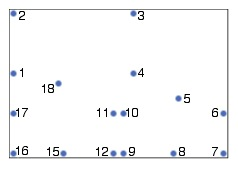
\includegraphics[scale=0.8]{LoudspeakerPositions}}
%\caption{Points represent positions of the 16 speakers used in the examples below.}
%\label{speaker_positions}
%\end{figure}

A visual representation of the behavior of the algorithm has been developed, using gradients to illustrate the ``predominance'' zone of each speaker. This is also intended to offer intuitive interactive manipulation of source positions and parameters such as spatial blur, rolloff and speaker weights.

\begin{figure}[ht]
\centerline{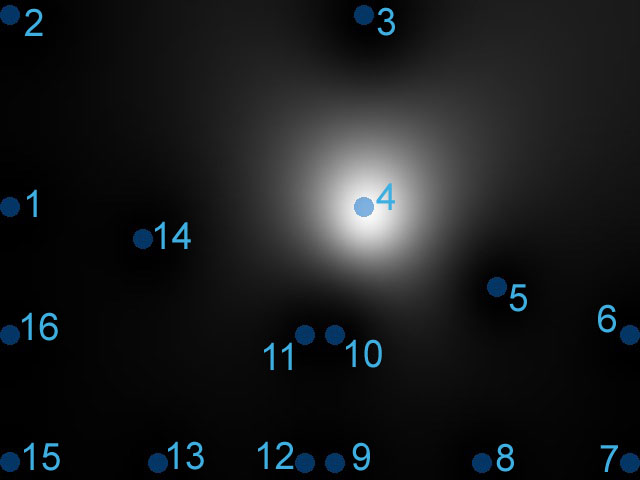
\includegraphics[scale=0.5]{spk4_r_6_b_0+nbrs}}
\caption{{Representation of the levels 2D distribution for speaker 4. Points represent positions of the 16 speakers.}}  
\label{fig:1spk}
\end{figure}

% Does this look better ?
% Tim says 'yes, good enough for now'

The method for creating this visualization consists in creating a graphical map of level response for each loudspeaker as a 2D matrix of levels. For each pixel of this matrix, the pixel value is set to the squared amplitude returned by the DBAP algorithm if the source was located at this position. The visual result in figure \ref{fig:1spk} indicates the spatial response for one of the loudspeakers. The lighter pixels are positions where amplitudes are close to $1$ and the darker pixels are positions where amplitudes are close to $0$. As expected, the further away the source is from the loudspeaker the lower the amplitude. 
%However the presence of holes in the spatial distribution of the amplitude response illustrates how the DBAP algorithm works when a source moves between several loudspeakers.
%This part above isn't really necessary

% CHANGED: Tim may not know what he is talking about, but he thinks the numbers for the dB values look odd in the PDF.  The 6 dB in particular.  Ignore if you think he's nuts. Pascal agrees and suggests removing the dollar signs just in case it could look better, so he'll try that out, and let's see how it turns out

%\begin{figure}[ht]
%\centerline{
\includegraphics[scale=0.5]{all_r_2_b_0}}
%\caption{{Representation of the 2D distribution of levels for all speakers. Parameter values are 2 dB for rolloff, and 0 for blur.}}  
%\label{fig:allspk1}
%\end{figure}

\begin{figure}[ht]
\centerline{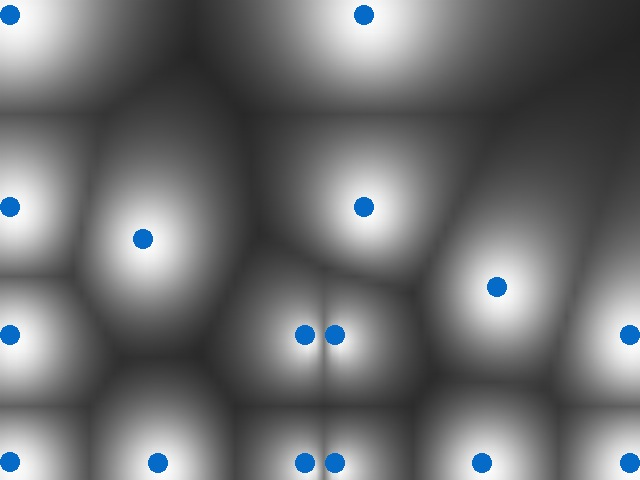
\includegraphics[scale=0.5]{all_r_6_b_0}}
\caption{Representation of the 2D distribution of levels for all speakers.}  
\label{fig:allspk2}
\end{figure}
%\begin{figure}[ht]
%\centerline{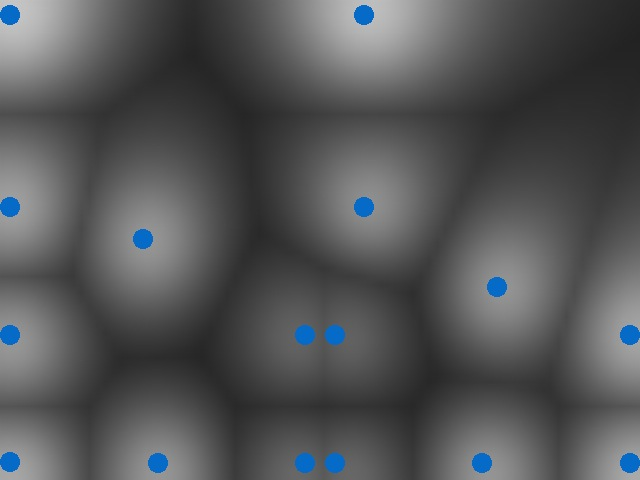
\includegraphics[scale=0.5]{all_r_6_b_0_2}}
%\caption{{\it Representation of the 2D distribution of levels for all speakers. Parameter values are 6 dB for rolloff, and 0.2 for blur}}  
%\label{fig:allspk3}
%\end{figure}
A visualization of the response ranges for all speakers can be created by combining all figures of the same class as in fig. \ref{fig:1spk}, and then finding the maximum amplitude for a given 2D-position. The graphical result, as in \ref{fig:allspk2}, shows segmented parts in space corresponding to every spatial zone of predominance for each loudspeaker. Here the darker pixels have to be explained as positions where the source is mixed equally between the closest loudspeakers. %Figures \ref{fig:allspk1}, \ref{fig:allspk2} and \ref{fig:allspk3} illustrate several combinations of varying roll off and blur values. 

\begin{figure}[ht]
\centerline{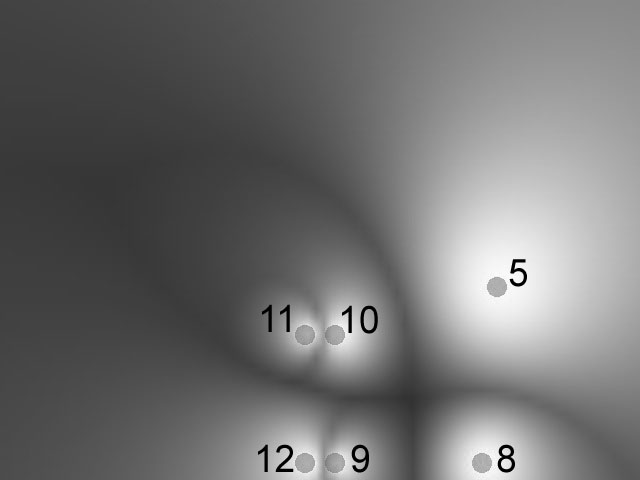
\includegraphics[scale=0.5]{spk_groups+nbrs}}
\caption{Representation of the 2D distribution of levels for 5 speakers only, with weights $[1.5,1.,1.,1.,0.75,1.2]$ for speakers $[5,8,9,10,11,12]$.}
\label{fig:5spk_weights}
\end{figure}
% Figure \ref{fig:5spk_weights} illustrates a weights preset that keeps only five loudspeakers set with different weights for each of them.
These pictures are generated in realtime by the algorithm, and may serve as a user-interface for source positioning and DBAP parameter setting.  Examples of this include use as back drops for mouse interaction or tactile-screen interaction.


\section{Conclusions and Further Work}

DBAP offers a light-weight panning-based solution for spatialization using irregular loudspeaker layouts. The Jamoma module implementation makes DBAP available with an interface similar to other Jamoma modules for rendering spatial sound, enabling various techniques to be interchanged and compared. %Jamoma also offers a more advanced spatialization technique that can be used for irregular loudspeaker layouts, ViMiC, incorporating distance-based signal delays between speakers, simulation of microphone patterns, early reflections and surface absorption \cite{Peters:2008vimic}. ViMiC is more CPU-intensive, and might require a dedicated computer for spatialization or limitations on the number of loudspeakers used as compared to DBAP.

Implementation of convex hulls and speaker weights remains to be combined (in the case of speakers subsets), and extended for three-dimensional loudspeaker layouts. 
%If speaker weights are used to define subspaces of speakers, it also remains to be investigated if and how the implementation of convex hulls can be dynamically reconfigured.

%In this paper DBAP has been discussed for spatialization to a static layout of speakers. For gaming applications the speaker layout relative to the player could be defined, and then the actual speaker layout could be changed dynamically as the gamer moves through the virtual world of the game.

DBAP can also be used as a solution for dynamic routing of input sources to a spatial layout of effect processes. Instead of defining loudspeaker positions, the effects could be assigned positions in a data space, similarly to
%. The idea of having sources traverse a space of effects would resemble e.g. the work by 
\cite{Momeni:2003hipnoscope}. 
%A project for designing multi-touch graphical interfaces to intuitively interact with DBAP has been initiated.


\section{Acknowledgements}

Initial development of DBAP was done for the workshop and exhibition ``Living room'' at Galleri KiT in Trondheim, 2003, produced by PNEK. Initial implementation in C of the DBAP algorithm was done by Andr\'e Sierr. The authors would like to express their gratitude to the other Jamoma developers, in particular Mathieu Chamagne for extensive and valuable feedback and Tim Place for proof-reading. 



\bibliographystyle{IEEEtranS}
\bibliography{icmc2009-dbap} % requires file template.bib

\end{document}

%
%This is the template file for the proceedings of the 9$^{th}$ International Conference on Digital Audio Effects (DAFx-06). 
%This template has been generated from WASPAA'99 templates and aims at producing conference proceedings in electronic form. 
%The format is essentially the one used for ICASSP conferences.

%Please use either this \LaTeX{} or the accompanying Word formats when preparing your submission. 
%The templates are available in electronic form at the website:
%\\ \href{http://www.dafx.ca}{http://www.dafx.ca}. Thanks!

%

%
%This template can be found on the conference website.

%\subsection{Figures} 
%All figures should be centered on the column (or page, if the figure spans both columns). 
%Figure captions (in italic) should follow each figure and have the format given in Figure \ref{fft_plot}.
%\begin{figure}[ht]
%\centerline{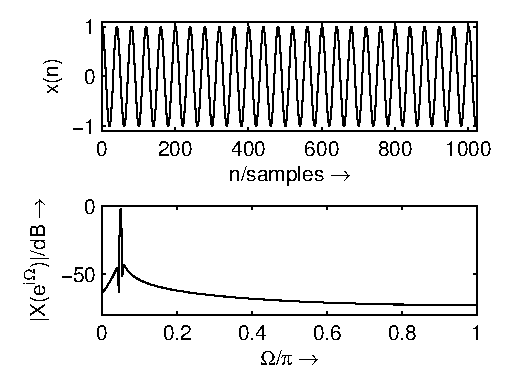
\includegraphics[scale=0.8]{fft_plot2}}
%\caption{{\it Sinusoid in time and frequency domain.}}  
%\label{fft_plot}
%\end{figure}
%Figures must be vectorial (no screen copy, no bitmap, etc). For example when using \texttt{Matlab}, export using either Postscript or PDF format. Also, in order to provide a better readibility, figure text font size should be at list identical to footnote font size. To do so using \texttt{Matlab}, use the \texttt{subplot} command before plotting.

%\subsection{Tables} 
%As for figures, all tables should be centered on the column (or page, if the table spans both columns). 
%Table captions should be in italic, follow each table and have the format given in Table \ref{tab:example}.

%\begin{table}[htdp]
%  \begin{center}
%    \begin{tabular}{|c|c|}\hline
%    	angle ($\theta$, rad) & $\sin \theta$ \\\hline
%	$\frac{\pi}{2}$ & 1 \\
%	$\pi$ & 0 \\
%	$\frac{3\pi}{2}$ & -1 \\
%	$2\pi$ & 0 \\\hline
%    \end{tabular}
%  \end{center}
%  \label{tab:example}
%  \caption{{\it Basic trigonometric values.}}
%\end{table}%

%\subsection{Equations}
%Equations should be placed on separate lines and numbered:

%\begin{equation}
%X(e^{j\Omega})=\sum_{n=0}^{N-1}x(n)e^{-j\Omega n}
%\label{eq1}
%\end{equation}
%where the sequence $x(n)$ in equation (\ref{eq1}) is a windowed frame:
%\begin{equation}
%x(n)=s(n)\cdot w(n)
%\label{eq2}
%\end{equation}
%with a window function $w(n)$.

%\subsection{Page Numbers}
%Page numbers will be added to the document electronically, so {\em please leave the numbering as is},
%that is, the first page will start at page DAFX-1 and the last page, at most, will have to be DAFX-6
%for the submission of papers for an oral presentation or DAFX-4 in the case of a poster presentation.

%\subsection{References}
%The references will be numbered in order of appearance \cite{Mitra:Kaiser:1993:DSP:handbook}, \cite{Haykin:1991:adaptive:filter}, \cite{Moorer:2000:AES:audio:millenium} and \cite{Arfib:1998:DAFx}. Please avoid listing references that do not appear in the text (we did the opposite in this template).

%\subsubsection{Reference Format}
%The reference format is the standard IEEE one. We recommend to use BibTeX to create the reference list.

%\section{Conclusions}
%This template can be found on the conference website. 
%If you wish to include two authors' affiliations please use the companion LaTeX template tmpl\_la2\_href. 
%Please, submit full-length papers (max.~6 pages for oral presentation and max.~4 pages for posters).
% 
%Submission is fully electronic and automated through the Conference Web Submission System. 
%DO NOT send us papers directly by e-mail. 

%\section{Acknowledgements}
%Many thanks to the great number of anonymous reviewers!

%%\newpage
%\nocite{*}
%\bibliographystyle{IEEEbib}
%\bibliography{template} % requires file template.bib

%\end{document}
